
% Copyright (c) 2015 - 2020 Mario Mlačak, mmlacak@gmail.com
% Licensed and published as Public Domain work.

% Discovery chapter ===================================================
\chapter*{Discovery}
\addcontentsline{toc}{chapter}{Discovery}
\label{ch:Discovery}

\begin{flushright}
\parbox{0.8\textwidth}{
\emph{I don't believe in God but I'm very interested in her. \\
\hspace*{\fill}{\textperiodcentered \textperiodcentered \textperiodcentered \hspace*{0.2em} Arthur C. Clarke} } }
\end{flushright}

\noindent
Discovery is chess variant which is played on 24 x 24 board, with
light (pastel!) yellow and gray fields and darker gray and dark teal
pieces. Star colors are bright orange and dark violet. In algebraic
notation, columns are enumerated from 'a' to 'x', and rows are
enumerated from '1' to '24'. A new piece is introduced, Monolith.

\clearpage % ..........................................................
% Monolith ************************************************************

\section*{Monolith}
\addcontentsline{toc}{section}{Monolith}
\label{sec:Discovery/Monolith}

\vspace*{-1.1\baselineskip}
\noindent
\begin{wrapfigure}[11]{l}{0.4\textwidth}
\centering
\includegraphics[width=0.4\textwidth, keepaspectratio=true]{pieces/17_monolith.png}
\caption{Monolith}
\label{fig:17_monolith}
\end{wrapfigure}
Monolith does not belong to any player, but can be moved by both of them.
Monolith cannot be captured, converted, activated, or displaced.
Pawns cannot be promoted to Monolith.

Monolith is a teleportation device, much like moveable Star. Piece can
initiate teleportation either by touching a Monolith or a field at which
it stands.

Piece, if not Wave, then reappears on a chosen empty portal-field around
any Star or the other Monolith. Wave teleported from a Monolith can emerge
only from the other Monolith. Kings, Monoliths cannot be teleported.

Piece teleported from a Star, if not Wave, can reappear on a chosen empty
portal-field around the 2 Stars in opposite color, or around any Monolith.
Wave teleported from a Star can only emerge from the other Star in the same
color.

Monolith cannot interact with (capture, activate, ...) any piece on its own;
all of its step-fields must be empty. Each step of a Monolith is longer
Knight-like jump than in a previous step. Monolith can make limited number of
steps, depending how many Pawns are owned by a player moving that Monolith.

Alternative move for Monolith is syzygy.

In algebraic notation, symbol for Monolith is 'M'.

\clearpage % ..........................................................

% \vspace*{0.05\textheight}
\noindent
\begin{wrapfigure}[2]{l}{0.4\textwidth}
\centering
\includegraphics[width=0.4\textwidth, keepaspectratio=true]{pieces/bishop/20_discovery.png}
\caption{Bishop}
\label{fig:bishop/20_discovery}
\end{wrapfigure}
Piece colors in this variant are presented on the left.

\vspace*{0.30\textheight}
\noindent
\begin{wrapfigure}[2]{l}{0.4\textwidth}
\centering
\includegraphics[width=0.4\textwidth, keepaspectratio=true]{pieces/star/20_discovery.png}
\caption{Star}
\label{fig:star/20_discovery}
\end{wrapfigure}
Star colors in this variant are presented on the left.

\clearpage % ..........................................................
% Movement ------------------------------------------------------------

\subsection*{Movement}
\addcontentsline{toc}{subsection}{Movement}
\label{sec:Discovery/Monolith/Movement}

\vspace*{-1.4\baselineskip}
\noindent
\begin{figure}[!h]
\includegraphics[width=1.0\textwidth, keepaspectratio=true]{examples/20_d/scn_d_01_monolith_patterns.png}
\vspace*{-1.3\baselineskip}
\caption{Diamond-shaped patterns}
\label{fig:scn_d_01_monolith_patterns}
\end{figure}

\vspace*{-0.5\baselineskip}
Monolith has its first step the same as Knight's, each consecutive step is slightly
longer than previous. Here, step-fields of starting Monolith's steps are marked; blue
for first step, grey for second, red for third, and green for fourth. All step-fields
are always in a color opposite to the color of Monolith's current field. Taken together,
step-fields of a single step form a diamond-shaped pattern. Pattern growth is not
limited, Monolith can take steps beyond the four shown here.

\clearpage % ..........................................................

\vspace*{-2.1\baselineskip}
\noindent
\begin{figure}[!h]
\includegraphics[width=1.0\textwidth, keepaspectratio=true]{examples/20_d/scn_d_02_monolith_first_step.png}
\vspace*{-1.3\baselineskip}
\caption{Monolith's first step}
\label{fig:scn_d_02_monolith_first_step}
\end{figure}

\vspace*{-0.5\baselineskip}
Monolith does not belong to any player, and can be moved by either. Step-fields
of Monolith's first step are identical to Knight's. Monolith cannot interact with
pieces at all; so, a step-field must be empty for a Monolith to step onto it.
Monolith is not restrained by any piece outside of its step-fields. \newline
\indent
Here, Monolith on its first step is blocked by two Waves, so cannot access already
occupied step-fields. This is so, regardless if light or dark player is moving a
Monolith.

\clearpage % ..........................................................

\vspace*{-2.1\baselineskip}
\noindent
\begin{figure}[!h]
\includegraphics[width=1.0\textwidth, keepaspectratio=true]{examples/20_d/scn_d_03_monolith_second_step.png}
\vspace*{-1.3\baselineskip}
\caption{Monolith's second step}
\label{fig:scn_d_03_monolith_second_step}
\end{figure}

\vspace*{-0.5\baselineskip}
In this, and next two examples grey arrows show path covered by Monolith in previous
steps, from its starting field M. For Monolith's second step, step-fields are identical
to \hyperref[fig:scn_aoa_02_unicorn_opposite_color]{Unicorn's long jump}; step-fields
of first step are enumerated. \newline
\indent
Step-fields are always in color opposite to current Monolith's field; each new step
is slightly larger, and covers fields neighboring to previous step; so, every new
diamond-shaped pattern has its sides longer by two fields.

% \TODO

% Taken together, step-fields form a diamond-shaped pattern. For each succeeding step,
% step-fields form slightly larger pattern than in preceding step. Step-fields of all
% patterns (steps) are always in a color opposite to a color of Monolith's current
% field. New, larger diamond-shaped pattern contains fields neighbouring step-fields
% of preceding step, and additionaly two more fields on each of its four sides.

\clearpage % ..........................................................

\vspace*{-2.1\baselineskip}
\noindent
\begin{figure}[!h]
\includegraphics[width=1.0\textwidth, keepaspectratio=true]{examples/20_d/scn_d_04_monolith_third_step.png}
\vspace*{-1.3\baselineskip}
\caption{Monolith's third step}
\label{fig:scn_d_04_monolith_third_step}
\end{figure}

\vspace*{-0.5\baselineskip}
Here, step-fields of a Monolith's third step are marked; step-fields of a second
step are enumerated. New diamond-shaped pattern contains fields neighbouring
previous pattern, and is larger by two fields on all four sides. \newline
\indent
Again, any empty step-field can be chosen freely, regardless of any previous choice.
Monolith is not obstructed by any piece that is not sitting in its step-fields.
Here, four step-fields are blocked by both light and dark pieces, equally so for
either light or dark player moving a Monolith.

\clearpage % ..........................................................

\vspace*{-2.1\baselineskip}
\noindent
\begin{figure}[!h]
\includegraphics[width=1.0\textwidth, keepaspectratio=true]{examples/20_d/scn_d_05_monolith_fourth_step.png}
\vspace*{-1.3\baselineskip}
\caption{Monolith's fourth step}
\label{fig:scn_d_05_monolith_fourth_step}
\end{figure}

\vspace*{-0.5\baselineskip}
Here, step-fields of a Monolith's fourth step are marked; step-fields of a third step
are enumerated. Again, new pattern is larger than previous by two fields on each side.
Each consecutive step has larger pattern, pattern growth is not limited. \newline
\indent
Number of steps Monolith can make is limited by how many Pawns are owned by a player
moving that Monolith. Here, Monolith moved by light player can take fourth step;
should it be moved by dark player only first two steps would be allowed.

\clearpage % ..........................................................

\subsubsection*{Off-board Monolith}
\addcontentsline{toc}{subsubsection}{Off-board Monolith}
\label{sec:Discovery/Monolith/Movement/Off-board Monolith}

\vspace*{-1.4\baselineskip}
\noindent
\begin{figure}[!h]
\includegraphics[width=1.0\textwidth, keepaspectratio=true]{examples/20_d/scn_d_06_monolith_off_board.png}
\vspace*{-1.3\baselineskip}
\caption{Monolith off-board}
\label{fig:scn_d_06_monolith_off_board}
\end{figure}

\vspace*{-0.4\baselineskip}
Here, light grey fields are virtual fields extending existing chessboard.
Monolith, similarly to \hyperref[fig:scn_hd_06_centaur_off_board]{Centaur},
cannot leave chessboard, and all subsequent steps are also illegal.

\clearpage % ..........................................................

\subsubsection*{Monolith is noble}
\addcontentsline{toc}{subsubsection}{Monolith is noble}
\label{sec:Discovery/Monolith/Movement/Monolith is noble}

\vspace*{-1.4\baselineskip}
\noindent
\begin{figure}[!h]
\includegraphics[width=1.0\textwidth, keepaspectratio=true]{examples/20_d/scn_d_07_monolith_is_noble.png}
\vspace*{-1.3\baselineskip}
\caption{Monolith is noble}
\label{fig:scn_d_07_monolith_is_noble}
\end{figure}

\vspace*{-0.4\baselineskip}
Image above have four examples in parallel; each in its own corner.

Monolith cannot be captured, converted, activated, or displaced. Pieces can only
teleport from a Monolith; except for Kings, Stars, and Monoliths which cannot
teleport.

\clearpage % ..........................................................

\subsubsection*{Trance-journey interaction}
\addcontentsline{toc}{subsubsection}{Trance-journey interaction}
\label{sec:Discovery/Monolith/Teleporting/Trance-journey interaction}

\vspace*{-1.4\baselineskip}
\noindent
\begin{figure}[!h]
\includegraphics[width=1.0\textwidth, keepaspectratio=true]{examples/20_d/scn_d_08_monolith_shaman_interaction.png}
\vspace*{-1.3\baselineskip}
\caption{Trance-journey interaction}
\label{fig:scn_d_08_monolith_shaman_interaction}
\end{figure}

\vspace*{-0.4\baselineskip}
Like with Stars (and Kings) in
\hyperref[fig:scn_cot_21_light_light_shaman_interaction_start]{the previous variant},
entranced Shamans cannot interact with Monolith, but can continue to move past it.
This is so regardless of colors of both entrancing (S) and entranced (T) Shamans.
Here, entranced light Shaman can displace dark Knight, which it can reach after
passing all non-interacting pieces.

\clearpage % ..........................................................

\subsubsection*{Monolith is opaque}
\addcontentsline{toc}{subsubsection}{Monolith is opaque}
\label{sec:Discovery/Monolith/Movement/Monolith is opaque}

\vspace*{-1.4\baselineskip}
\noindent
\begin{figure}[!h]
\includegraphics[width=1.0\textwidth, keepaspectratio=true]{examples/20_d/scn_d_09_monolith_is_opaque.png}
\vspace*{-1.3\baselineskip}
\caption{Monolith is opaque}
\label{fig:scn_d_09_monolith_is_opaque}
\end{figure}

\vspace*{-0.4\baselineskip}
Image above have two examples in parallel; at the top, and to the bottom.

Monolith is opaque; no piece can "pass-through" Monolith, neither material pieces,
nor Waves. Here, light Bishop cannot capture dark Pawn, because Monolith B is in
the way. Similarly, light Wave cannot activate Queen, since Monolith A is between
the two.

% ------------------------------------------------------------ Movement
\clearpage % ..........................................................
% Teleporting ---------------------------------------------------------

\subsection*{Teleporting}
\addcontentsline{toc}{subsection}{Teleporting}
\label{sec:Discovery/Monolith/Teleporting}

\vspace*{-1.4\baselineskip}
\noindent
\begin{figure}[!h]
\includegraphics[width=1.0\textwidth, keepaspectratio=true]{examples/20_d/scn_d_10_teleport_via_monolith.png}
\vspace*{-1.3\baselineskip}
\caption{Teleporting piece via Monolith}
\label{fig:scn_d_10_teleport_via_monolith}
\end{figure}

\vspace*{-0.4\baselineskip}
Teleportation using Monoliths is similar to one using Stars in \hyperref[fig:scn_n_02_teleport_init]{previous variant, Nineteen}.
Pieces, if not Waves, teleporting from Monolith can reappear near any Star or the other Monolith.
All momentum carried is lost. Again, Kings and Monoliths cannot be teleported.
Here, all empty portal-fields where Bishop can be teleported to are enumerated.

\clearpage % ..........................................................

\noindent
\begin{figure}[!h]
\includegraphics[width=1.0\textwidth, keepaspectratio=true]{examples/20_d/scn_d_11_teleport_via_star.png}
\vspace*{-1.3\baselineskip}
\caption{Teleporting piece via Star}
\label{fig:scn_d_11_teleport_via_star}
\end{figure}

\vspace*{-0.4\baselineskip}
All pieces, except Waves, teleporting from a Star can reappear on a empty portal-field
near Stars in opposite color, or near any Monolith.
Here, all empty portal-fields where Bishop can be teleported to are enumerated.

\clearpage % ..........................................................
% Teleporting Wave ....................................................

\subsubsection*{Teleporting Wave}
\addcontentsline{toc}{subsubsection}{Teleporting Wave}
\label{sec:Discovery/Monolith/Teleporting/Teleporting Wave}

\vspace*{-1.4\baselineskip}
\noindent
\begin{figure}[!h]
\includegraphics[width=1.0\textwidth, keepaspectratio=true]{examples/20_d/scn_d_12_teleport_wave_via_star.png}
\vspace*{-1.3\baselineskip}
\caption{Teleporting Wave via Star}
\label{fig:scn_d_12_teleport_wave_via_star}
\end{figure}

\vspace*{-0.4\baselineskip}
Teleporting Wave using Star is the same as in \hyperref[fig:scn_n_04_teleport_move_3]{previous variant, Nineteen}.
Wave teleported from a Star emerges from the other Star in the same color,
and continues to move from position of a destination Star in the same
direction as before teleportation. Teleported Wave retains momentum carried.
Here, light Wave could activate own Bishop after teleporting with 2 momentum.

\clearpage % ..........................................................

\vspace*{-2.3\baselineskip}
\noindent
\begin{figure}[!h]
\includegraphics[width=1.0\textwidth, keepaspectratio=true]{examples/20_d/scn_d_13_teleport_wave_via_monolith.png}
\vspace*{-1.3\baselineskip}
\caption{Teleporting Wave via Monolith}
\label{fig:scn_d_13_teleport_wave_via_monolith}
\end{figure}

\vspace*{-0.3\baselineskip}
Wave teleported from a Monolith emerges from the other Monolith, and continues
movement from position of a destination Monolith in the same direction as before
teleportation, while retaining momentum carried into teleportation.
Here, light Wave could activate own Bishop after teleporting with 2 momentum. \newline
Since \hyperref[fig:scn_d_09_monolith_is_opaque]{Monolith is opaque}, Wave cannot
pass beyond it, as it can do with all the other pieces. So, teleportation is
mandatory for Wave when it reaches Monolith.

\clearpage % ..........................................................

\vspace*{-2.3\baselineskip}
\noindent
\begin{figure}[!h]
\includegraphics[width=1.0\textwidth, keepaspectratio=true]{examples/20_d/scn_d_14_teleported_wave_blocked.png}
\vspace*{-1.3\baselineskip}
\caption{Teleported Wave blocked}
\label{fig:scn_d_14_teleported_wave_blocked}
\end{figure}

\vspace*{-0.3\baselineskip}
In case where all step-fields of a teleported Wave are blocked, it is oblationed, like in
\hyperref[fig:scn_n_06_teleport_wave_blocked]{previous variant, Nineteen}. \newline
\hyperref[fig:scn_n_03_teleport_move_2]{The same applies to all other material (i.e. non-Wave) pieces}.
If all portal-fields where teleported piece could reappear are occupied, piece is removed
from chessboard. \newline
Here, Wave cannot neither activate light Queen, nor reach any step-fields beyond Monolith;
Wave has to teleport when it reaches Monolith.

\clearpage % ..........................................................

\vspace*{-1.4\baselineskip}
\noindent
\begin{figure}[!h]
\includegraphics[width=1.0\textwidth, keepaspectratio=true]{examples/20_d/scn_d_15_wave_teleported_off_board.png}
\vspace*{-1.3\baselineskip}
\caption{Wave teleported off-board}
\label{fig:scn_d_15_wave_teleported_off_board}
\end{figure}

\vspace*{-0.3\baselineskip}
Teleported Wave with all of its step-fields located off-board is also oblationed.

\clearpage % ..........................................................

\vspace*{-1.4\baselineskip}
\noindent
\begin{figure}[!h]
\includegraphics[width=1.0\textwidth, keepaspectratio=true]{examples/20_d/scn_d_16_wave_teleport_on_and_off_board.png}
\vspace*{-1.3\baselineskip}
\caption{Teleporting Wave on- and off-board}
\label{fig:scn_d_16_wave_teleport_on_and_off_board}
\end{figure}

\vspace*{-0.3\baselineskip}
Before and after teleportation, Wave can step outside of a board, as long as its ply ends
on a board. Like in \hyperref[fig:scn_n_08_teleport_wave_end]{previous variant, Nineteen},
Wave has to continue alternating steps after teleportation; if teleported off with up-right
step, Wave has to emerge from the other Monolith with up-left step. Here, light Wave could
also activate own Bishop after teleportation with 3 momentum, or have a teleportation cascade.

% .................................................... Teleporting Wave
\clearpage % ..........................................................

\subsubsection*{Teleportation cascade}
\addcontentsline{toc}{subsubsection}{Teleportation cascade}
\label{sec:Discovery/Monolith/Teleporting/Teleportation cascade}

\vspace*{-0.9\baselineskip}
\noindent
\begin{figure}[!h]
\includegraphics[width=1.0\textwidth, keepaspectratio=true]{examples/20_d/scn_d_17_teleporting_wave_cascade.png}
\vspace*{-1.3\baselineskip}
\caption{Cascading teleportations}
\label{fig:scn_d_17_teleporting_wave_cascade}
\end{figure}

\vspace*{-0.3\baselineskip}
Teleportation cascade refers to Wave being teleported at least twice in the same ply;
other pieces can't cascade teleportations. Unlike in a previous variants, thanks to
Monolith, teleportation cascade is now useful in granting access to otherwise unreachable
places. Here, light Wave can activate own Bishop only after second teleportation
(A $\rightarrow$ B, then C $\rightarrow$ D).

\clearpage % ..........................................................
% Steps after Teleportation ...........................................

\subsubsection*{Steps after teleportation}
\addcontentsline{toc}{subsubsection}{Steps after teleportation}
\label{sec:Discovery/Monolith/Teleporting/Steps after teleportation}

\vspace*{-1.4\baselineskip}
\noindent
\begin{figure}[!h]
\includegraphics[width=1.0\textwidth, keepaspectratio=true]{examples/20_d/scn_d_18_steps_after_teleport_init.png}
\vspace*{-1.3\baselineskip}
\caption{Steps before teleportation}
\label{fig:scn_d_18_steps_after_teleport_init}
\end{figure}

\vspace*{-0.3\baselineskip}
Wave, \hyperref[fig:scn_mv_22_wave_activation_by_unicorn_first_step]{activated by Unicorn}
(\hyperref[fig:scn_hd_07_wave_activation_by_centaur_first_step]{or Centaur}), at the
beginning of a ply has to choose two different steps (long and short jump) depending
on a color of a step-fields; once chosen they can't be changed for the duration of
that ply. Teleported Wave, activated by Unicorn (or Centaur), still has to
\hyperref[fig:scn_n_07_teleport_wave_init]{follow two initially chosen steps},
\hyperref[fig:scn_n_09_teleport_wave_2_init]{according to a color of a field}
of emerging Star (or Monolith).

\clearpage % ..........................................................

\vspace*{-2.3\baselineskip}
\noindent
\begin{figure}[!h]
\includegraphics[width=1.0\textwidth, keepaspectratio=true]{examples/20_d/scn_d_19_steps_after_teleport_end.png}
\vspace*{-1.3\baselineskip}
\caption{Steps after teleportation}
\label{fig:scn_d_19_steps_after_teleport_end}
\end{figure}

\vspace*{-0.3\baselineskip}
Monoliths can be moved by both players, and they can be positioned on a fields in
opposite colors. If so, teleported Wave, activated by Unicorn (or Centaur), still
has to follow initially chosen steps; two-step pattern remains the same, only steps
are reversed, i.e. first step after emerging is the same as last step before
teleporting. \newline
Here, emerging step is the same as teleporting step (blue arrow); two-step pattern
otherwise is the same, only order of steps is reversed.

% ........................................... Steps after Teleportation
% --------------------------------------------------------- Teleporting
\clearpage % ..........................................................
% Syzygy --------------------------------------------------------------

\subsection*{Syzygy}
\addcontentsline{toc}{subsection}{Syzygy}
\label{sec:Discovery/Monolith/Syzygy}

\vspace*{-1.4\baselineskip}
\noindent
\begin{figure}[!h]
\includegraphics[width=1.0\textwidth, keepaspectratio=true]{examples/20_d/scn_d_20_syzygy_explain.png}
\caption{Syzygy with Stars}
\label{fig:scn_d_20_syzygy_explain}
\end{figure}

Syzygy is alignment in one straight line of at least 3 celestial bodies, Stars and
Monoliths. It's initiated by Monolith stepping onto horizontal, vertical or diagonal
line connecting 2 Stars. Syzygy-fields are all fields where Monolith would be in
syzygy. For horizontal and vertical syzygy, syzygy-fields are the same as Rook
step-fields; for diagonal syzygy, syzygy-fields are the same as Bishop step-fields.

\clearpage % ..........................................................

% \vspace*{-1.2\baselineskip}
\noindent
\begin{figure}[!h]
\includegraphics[width=1.0\textwidth, keepaspectratio=true]{examples/20_d/scn_d_21_syzygy_2_stars_init.png}
\caption{2-Stars syzygy start}
\label{fig:scn_d_21_syzygy_2_stars_init}
\end{figure}

Immediately after Monolith has stepped into syzygy, one own figure can then be (but
don't have to be) demoted to Pawn. Demoting to Pawn can be done even if no own Pawn
has been captured yet. Opponent pieces, Kings, Stars, Monoliths cannot be demoted.
Unlike promotion, demoting to Pawn cannot be saved for later. If player chooses to
demote own figure, it must happen in the very same move in which Monolith has
stepped into a syzygy.

\clearpage % ..........................................................

\noindent
\begin{figure}[!h]
\includegraphics[width=1.0\textwidth, keepaspectratio=true]{examples/20_d/scn_d_22_syzygy_2_stars_steps.png}
\caption{2-Stars syzygy steps}
\label{fig:scn_d_22_syzygy_2_stars_steps}
\end{figure}

If Monolith was moved into syzygy by light player, light Wave or Bishop could be
demoted (blue); if moved by dark player only dark Rook could be demoted (green).
Demoting to Pawn can only be done after Monolith stepped into alignment; once in
it, no additional figures can be demoted on subsequent turns. To demote again,
the same Monolith has to step outside of alignment in one move and then back in
another (or the other Monolith has to step-in).

\clearpage % ..........................................................
% Two-Monoliths syzygy ................................................

\subsubsection*{Two-Monoliths syzygy}
\addcontentsline{toc}{subsubsection}{Two-Monoliths syzygy}
\label{sec:Discovery/Monolith/Syzygy/Two-Monoliths syzygy}

\vspace*{-1.4\baselineskip}
\noindent
\begin{figure}[!h]
\includegraphics[width=1.0\textwidth, keepaspectratio=true]{examples/20_d/scn_d_23_syzygy_2_monoliths_init.png}
\caption{2-Monoliths syzygy init}
\label{fig:scn_d_23_syzygy_2_monoliths_init}
\end{figure}

For a Star and 2 Monoliths to be in syzygy there has to be a step which, when applied
repeatedly (from a Star) connects fields at which those celestial bodies are located.
Connecting step doesn't have to correspond to the movement of any piece, it's enough
if it connects celestial bodies. Shortest such a step is called syzygy-step, fields
which are connected by syzygy-steps are called syzygy-fields.

\clearpage % ..........................................................

\noindent
\begin{figure}[!h]
\includegraphics[width=1.0\textwidth, keepaspectratio=true]{examples/20_d/scn_d_24_syzygy_2_monoliths_steps.png}
\caption{2-Monoliths syzygy steps}
\label{fig:scn_d_24_syzygy_2_monoliths_steps}
\end{figure}

All own figures (except King) on a syzygy-fields are then eligible to be demoted
to Pawn. Here, there is a connecting step between fields 1-3 and 3-5. There is an
equivalent, shorter step connecting fields 1-2, 2-3, etc.; this is actual syzygy-step,
because it is the shortest one possible. Light Knight does lay on a syzygy-field, and
so is eligible to demotion, if Monolith was moved by light player.

% ................................................ Two-Monoliths syzygy
\clearpage % ..........................................................
% Reentering syzygy ...................................................

\subsubsection*{Reentering syzygy}
\addcontentsline{toc}{subsubsection}{Reentering syzygy}
\label{sec:Discovery/Monolith/Syzygy/Reentering syzygy}

\vspace*{-1.4\baselineskip}
\noindent
\begin{figure}[!h]
\includegraphics[width=1.0\textwidth, keepaspectratio=true]{examples/20_d/scn_d_25_syzygy_reentering_same_move.png}
\caption{Reentering syzygy in the same move}
\label{fig:scn_d_25_syzygy_reentering_same_move}
\end{figure}

To be granted option to demote own figure, Monolith must move from an ordinary, non-syzygy field into syzygy. It is
not enough if Monolith in a syzygy stepped out of alignment, and then back into it, in the very same move. Monolith
which is already in a syzygy can move into the same alignment, but cannot demote any figure.

\clearpage % ..........................................................

\noindent
\begin{figure}[!h]
\includegraphics[width=1.0\textwidth, keepaspectratio=true]{examples/20_d/scn_d_26_syzygy_reentering_independent.png}
\caption{Reentering independent syzygy}
\label{fig:scn_d_26_syzygy_reentering_independent}
\end{figure}

The same applies even if Monolith moves into an alignment from completely independent syzygy, i.e. even if the two does
not share neither any syzygy-fields nor celestial pieces.

In short, to get option to demote again, Monolith has to move out of alignment onto an ordinary, non-syzygy field in a
first move, and then on a next move Monolith can reenter the same syzygy, or enter the other syzygy.

% ................................................... Reentering syzygy
\clearpage % ..........................................................

\subsubsection*{In opponent's figure row}
\addcontentsline{toc}{subsubsection}{In opponent's figure row}
\label{sec:Discovery/Monolith/Syzygy/In opponent's figure row}

\vspace*{-1.4\baselineskip}
\noindent
\begin{figure}[!h]
\includegraphics[width=1.0\textwidth, keepaspectratio=true]{examples/20_d/scn_d_27_syzygy_in_opponents_figure_row.png}
\caption{Syzygy ends with Pawn tagged for promotion}
\label{fig:scn_d_27_syzygy_in_opponents_figure_row}
\end{figure}

Pawns which were demoted after syzygy in
\hyperref[sec:Terms/Figure row]{opponent's figure row}
are then either \hyperref[sec:Age of Aquarius/Promotion]{tagged for promotion},
or promoted straight away, in the same move, similar to
\hyperref[fig:scn_n_11_teleport_pawns_init]{previous variant, Nineteen}.

% -------------------------------------------------------------- Syzygy
% ************************************************************ Monolith
\clearpage % ..........................................................

\section*{Rush, en passant}
\addcontentsline{toc}{section}{Rush, en passant}
\label{sec:Discovery/Rush, en passant}

\vspace*{-1.4\baselineskip}
\noindent
\begin{figure}[!h]

\includegraphics[width=1.0\textwidth, keepaspectratio=true]{en_passants/20_discovery_en_passant.png}
\caption{En passant}
\label{fig:20_discovery_en_passant}
\end{figure}

Rush and en passant are identical to those in \hyperref[fig:14_hemera_s_dawn_en_passant]{Hemera's Dawn variant}.
Own Pawns can be rushed for up to 10 fields in this variant.

\clearpage % ..........................................................

\section*{Promotion}
\addcontentsline{toc}{section}{Promotion}
\label{sec:Discovery/Promotion}

Promotion is non enforced, delayed variety, i.e. it's the same as in
\hyperref[sec:Age of Aquarius/Promotion]{previous chess variant}, Age of Aquarius.

Promotion in this variant is polygamous, more than one Queen in the same color
can be present on chessboard at any given time.

Again, Pawn cannot be promoted to Monolith.

\clearpage % ..........................................................

\section*{Castling}
\addcontentsline{toc}{section}{Castling}
\label{sec:Discovery/Castling}

Castling is
\hyperref[sec:Nineteen/Castling]{the same as in Nineteen variant},
only difference is that King can move
between 2 and 9 fields across. All other constraints from Nineteen variant still
applies.

\noindent
\begin{figure}[!h]
\includegraphics[width=1.0\textwidth, keepaspectratio=true]{castlings/20_d/discovery_castling.png}
\caption{Castling}
\label{fig:discovery_castling}
\end{figure}

In example above, all valid King's castling moves are numbered.

\noindent
\begin{figure}[!h]
\includegraphics[width=1.0\textwidth, keepaspectratio=true]{castlings/20_d/discovery_castling_left_07.png}
\caption{Castling long left}
\label{fig:discovery_castling_left_07}
\end{figure}

In this example King was castling long to the left. Initial King's position is marked with "K".
After castling is finished, left Rook ends up at field immediately right to the King.

\clearpage % ..........................................................

\section*{Initial setup}
\addcontentsline{toc}{section}{Initial setup}
\label{sec:Discovery/Initial setup}

Compared to initial setup of Conquest of Tlalocan, just 2 Monoliths are placed in to the open,
symetrically, on both sides of chessboard. This can be seen in the image below:

\noindent
\begin{figure}[h]
\includegraphics[width=1.0\textwidth, keepaspectratio=true]{boards/20_discovery.png}
\caption{Discovery board}
\label{fig:20_discovery}
\end{figure}

\clearpage % ..........................................................
% =================================================== Discovery chapter
